%% IEEE Transactions on Medical Imaging
%% HSANet: Uncertainty-Aware Brain Tumor Classification
%% Using the IEEEtran class for journal submission

\documentclass[journal]{IEEEtran}

% Essential packages
\usepackage[utf8]{inputenc}
\usepackage[T1]{fontenc}
\usepackage{amsmath,amssymb,amsfonts}
\usepackage{algorithmic}
\usepackage{algorithm}
\usepackage{graphicx}
\usepackage{textcomp}
\usepackage{xcolor}
\usepackage{booktabs}
\usepackage{multirow}
\usepackage{cite}
\usepackage{url}
\usepackage{balance}
\usepackage{array}

% TikZ for figures
\usepackage{tikz}
\usetikzlibrary{shapes,arrows,positioning,fit,calc,backgrounds,decorations.pathreplacing,arrows.meta}
\usepackage{pgfplots}
\pgfplotsset{compat=1.17}

% Custom colors for architecture diagrams
\definecolor{backbone}{RGB}{66,133,244}
\definecolor{amsm}{RGB}{52,168,83}
\definecolor{dam}{RGB}{251,188,5}
\definecolor{edl}{RGB}{234,67,53}
\definecolor{feature}{RGB}{154,160,166}

% Hyperref (load last)
\usepackage{hyperref}
\hypersetup{
    colorlinks=true,
    linkcolor=blue,
    citecolor=blue,
    urlcolor=blue
}

% Correct bad hyphenation
\hyphenation{con-vo-lu-tion-al neu-ro-ra-di-ol-o-gy glio-blas-to-ma me-nin-gi-o-ma}

\begin{document}

% Paper title
\title{HSANet: A Hybrid Scale-Attention Network with Evidential Deep Learning for Uncertainty-Aware Brain Tumor Classification in MRI}

% Author information
\author{Md.~Assaduzzaman,~\IEEEmembership{Member,~IEEE,}
        Md.~Tareque~Jamil~Josh,~\IEEEmembership{Student~Member,~IEEE,}
        Md.~Aminur~Rahman~Joy,
        and~Md.~Nafish~Imtiaz~Imti%
\thanks{Manuscript received January 15, 2026; revised January 28, 2026; accepted January 30, 2026. Date of publication February XX, 2026; date of current version January 31, 2026. This work was supported by the Department of Computer Science and Engineering, Daffodil International University, Dhaka, Bangladesh. \textit{(Corresponding author: Md. Assaduzzaman.)}}%
\thanks{Md. Assaduzzaman is an Assistant Professor with the Department of Computer Science and Engineering, Daffodil International University, Daffodil Smart City, Ashulia, Dhaka 1341, Bangladesh (e-mail: assaduzzaman.cse@diu.edu.bd).}%
\thanks{Md. Tareque Jamil Josh, Md. Aminur Rahman Joy, and Md. Nafish Imtiaz Imti are undergraduate researchers with the Department of Computer Science and Engineering, Daffodil International University, Daffodil Smart City, Ashulia, Dhaka 1341, Bangladesh (e-mail: tarequecs@gmail.com).}%
\thanks{Code, pretrained models, and supplementary materials are publicly available at: \url{https://github.com/tarequejosh/HSANet-Brain-Tumor-Classification}}}

% Running header
\markboth{IEEE TRANSACTIONS ON MEDICAL IMAGING, VOL. XX, NO. XX, FEBRUARY 2026}%
{Assaduzzaman \MakeLowercase{\textit{et al.}}: HSANet for Uncertainty-Aware Brain Tumor Classification}

% Create title
\maketitle

% Abstract
\begin{abstract}
Accurate classification of brain tumors from magnetic resonance imaging (MRI) remains a fundamental challenge in computer-aided diagnosis, complicated by substantial morphological heterogeneity across tumor types and the absence of principled uncertainty quantification in conventional deep learning approaches. Current methods typically produce point predictions without meaningful confidence assessment, limiting their utility in safety-critical clinical workflows where knowing ``what the model doesn't know'' is as important as the prediction itself. We present HSANet, a hybrid scale-attention architecture that integrates adaptive multi-scale feature extraction with evidential learning for uncertainty-aware tumor classification. The proposed Adaptive Multi-Scale Module (AMSM) employs parallel dilated convolutions with content-dependent fusion weights, dynamically adjusting receptive fields to accommodate the substantial size variation observed across clinical presentations. A Dual Attention Module (DAM) applies sequential channel-then-spatial refinement to emphasize pathologically significant regions while suppressing irrelevant anatomical background. Critically, our evidential classification head replaces conventional softmax outputs with Dirichlet distributions, enabling decomposed uncertainty estimates that distinguish between inherent data ambiguity (aleatoric) and model knowledge limitations (epistemic). Comprehensive experiments on 7,023 brain MRI scans spanning four diagnostic categories demonstrate 99.77\% classification accuracy with excellent calibration (expected calibration error = 0.019). Misclassified samples exhibit significantly elevated epistemic uncertainty ($p < 0.001$, Mann-Whitney U test), confirming the clinical utility of uncertainty-guided decision support. Gradient-weighted class activation mapping validates attention on established radiological landmarks. Complete implementation and pretrained weights are publicly available.
\end{abstract}

% Keywords
\begin{IEEEkeywords}
Brain tumor classification, deep learning, uncertainty quantification, evidential deep learning, attention mechanism, multi-scale feature extraction, convolutional neural networks, medical image analysis.
\end{IEEEkeywords}

% Main body
\section{Introduction}

\IEEEPARstart{B}{rain} tumors represent one of the most challenging diagnostic entities in clinical oncology, with global surveillance data reporting approximately 308,102 new cases in 2020 alone~\cite{sung2021global}. The complexity of accurate diagnosis stems from the remarkable diversity of pathological entities---the 2021 World Health Organization (WHO) classification now recognizes over 100 distinct tumor types, each characterized by unique molecular fingerprints and clinical trajectories~\cite{louis2021who}. Prognostic outcomes vary dramatically across tumor categories: patients diagnosed with glioblastoma face a median survival of merely 14 to 16 months, whereas those with completely resected Grade I meningiomas frequently achieve long-term cure~\cite{ostrom2021cbtrus}. This substantial heterogeneity in clinical outcomes underscores the critical importance of precise tumor identification for treatment planning and patient counseling.

Magnetic resonance imaging (MRI) has become the cornerstone of neuro-oncological evaluation, providing superior soft-tissue contrast without ionizing radiation exposure~\cite{pope2018brain}. Expert neuroradiologists integrate multiparametric imaging findings with clinical presentation to formulate diagnoses. However, the global radiology workforce confronts escalating mismatches between imaging volume growth and specialist availability. Documented vacancy rates have reached 29\% in major healthcare systems, with projected shortfalls of 40\% anticipated by 2027~\cite{rimmer2017radiologist}. Interpretive fatigue has been implicated in diagnostic error rates of 3--5\% even among experienced specialists~\cite{bruno2015understanding}, motivating the development of computer-aided diagnostic systems to augment clinical workflows.

Over the past decade, deep convolutional neural networks (CNNs) have demonstrated considerable promise for automated medical image analysis, particularly when leveraging transfer learning from large-scale natural image datasets~\cite{krizhevsky2012imagenet,raghu2019transfusion}. Research groups worldwide have reported encouraging results for brain tumor classification, with reported accuracies typically ranging between 94\% and 99\% across various backbone architectures including VGG, ResNet, and the EfficientNet family~\cite{deepak2019brain,badvza2020classification,swati2019brain,aurna2022multiclass}. Despite these advances, several critical limitations prevent straightforward translation of existing methods into clinical practice.

First, brain tumors exhibit extraordinary morphological diversity spanning multiple orders of magnitude in spatial extent. Pituitary microadenomas may measure only 2--3 millimeters, whereas glioblastomas frequently exceed 5 centimeters with extensive peritumoral edema and mass effect. Standard convolutional architectures employ fixed receptive fields, creating inherent trade-offs between sensitivity to fine-grained textural features and capture of global contextual information. Second, brain MRI volumes contain extensive normal anatomical content that provides no diagnostic value yet dominates image statistics. Without explicit attention mechanisms, networks may learn spurious correlations with background tissue rather than genuine tumor characteristics. Third---and most critically for clinical deployment---conventional classifiers produce point predictions without meaningful confidence assessment. A network assigning 51\% probability to one class yields identical output as one with 99\% confidence, yet these scenarios demand fundamentally different clinical responses.

Recent advances in vision architectures have addressed some of these challenges. Multi-scale feature fusion strategies, such as Atrous Spatial Pyramid Pooling (ASPP)~\cite{chen2018encoder}, enable capture of context at multiple spatial scales. Attention mechanisms, including the Convolutional Block Attention Module (CBAM)~\cite{woo2018cbam} and Squeeze-and-Excitation networks~\cite{hu2018squeeze}, have demonstrated effectiveness for emphasizing relevant features while suppressing noise. However, the integration of these architectural innovations with principled uncertainty quantification remains underexplored in medical imaging applications.

Uncertainty quantification is particularly important for safety-critical medical applications where misdiagnosis carries significant consequences. Conventional approaches to uncertainty estimation, such as Monte Carlo dropout~\cite{gal2016dropout} and deep ensembles~\cite{lakshminarayanan2017simple}, require multiple forward passes during inference, substantially increasing computational costs and limiting real-time deployment. Evidential deep learning~\cite{sensoy2018evidential} has emerged as an alternative framework that places Dirichlet priors over categorical distributions, enabling single-pass uncertainty estimation with natural decomposition into aleatoric (data-inherent) and epistemic (model-knowledge) components.

In this work, we propose HSANet (Hybrid Scale-Attention Network), a novel architecture that addresses the aforementioned limitations through three key contributions:

\begin{enumerate}
\item An \textbf{Adaptive Multi-Scale Module (AMSM)} that captures tumor features across multiple spatial scales through parallel dilated convolutions with input-adaptive fusion weights. Unlike fixed multi-scale approaches, AMSM learns to weight different receptive fields based on input content, enabling effective feature extraction for both small and large tumors.

\item A \textbf{Dual Attention Module (DAM)} that implements sequential channel-then-spatial attention refinement. The channel attention component identifies diagnostically relevant feature channels, while the spatial attention component highlights tumor regions while suppressing irrelevant anatomical background.

\item An \textbf{evidential classification head} based on Dirichlet distributions that provides principled uncertainty estimates from a single forward pass. The framework decomposes total predictive uncertainty into aleatoric and epistemic components, enabling clinically meaningful confidence assessment.
\end{enumerate}

Comprehensive experiments on a challenging four-class brain tumor benchmark demonstrate that HSANet achieves 99.77\% classification accuracy while providing well-calibrated uncertainty estimates. Importantly, misclassified samples exhibit significantly elevated epistemic uncertainty, confirming that the model appropriately flags uncertain predictions for expert review. Gradient-weighted Class Activation Mapping (Grad-CAM) visualizations validate that learned attention patterns align with established neuroradiological diagnostic criteria.

The remainder of this paper is organized as follows. Section~\ref{sec:related} reviews related work in brain tumor classification and uncertainty quantification. Section~\ref{sec:methods} presents the HSANet architecture in detail. Section~\ref{sec:experiments} describes experimental setup and evaluation methodology. Section~\ref{sec:results} presents comprehensive results and analysis. Section~\ref{sec:discussion} discusses clinical implications and limitations. Section~\ref{sec:conclusion} concludes the paper.


\section{Related Work}
\label{sec:related}

\subsection{Deep Learning for Brain Tumor Classification}

The application of deep learning to brain tumor classification has progressed substantially over the past decade. Early approaches employed shallow CNN architectures trained from scratch on relatively small datasets, with limited generalization capability~\cite{mohsen2018classification}. The advent of transfer learning from ImageNet-pretrained models substantially improved performance, with VGG and ResNet architectures demonstrating strong results on brain MRI analysis~\cite{swati2019brain,badvza2020classification}.

Deepak and Ameer~\cite{deepak2019brain} proposed a two-stage approach using GoogLeNet for feature extraction followed by SVM classification, achieving 98.0\% accuracy on a three-class tumor dataset. Rehman \textit{et al.}~\cite{rehman2020deep} systematically compared VGG-16, ResNet-50, and GoogLeNet for brain tumor classification, reporting 98.87\% accuracy with fine-tuned VGG-16. More recent work has leveraged the EfficientNet family~\cite{tan2019efficientnet}, which achieves favorable accuracy-efficiency trade-offs through compound scaling of network width, depth, and resolution. Aurna \textit{et al.}~\cite{aurna2022multiclass} applied EfficientNet-B0 to four-class tumor classification, achieving 98.87\% accuracy.

Several studies have explored hybrid approaches combining CNNs with handcrafted features or classical machine learning classifiers~\cite{kibriya2022novel}. Attention mechanisms have been incorporated to improve feature discrimination, with squeeze-and-excitation blocks~\cite{hu2018squeeze} and self-attention layers~\cite{saeedi2023mri} demonstrating benefits for tumor classification. However, these approaches typically employ attention for accuracy improvement without addressing uncertainty quantification.

\subsection{Multi-Scale Feature Extraction}

The substantial size variation among brain tumors motivates multi-scale feature extraction strategies. Atrous (dilated) convolutions~\cite{yu2016multi} expand receptive fields without increasing parameters, enabling capture of context at multiple spatial scales. ASPP~\cite{chen2018encoder} employs parallel atrous convolutions with different dilation rates, followed by concatenation and fusion, achieving strong results in semantic segmentation tasks.

In medical imaging, multi-scale approaches have been applied to various modalities. Feature pyramid networks~\cite{lin2017feature} aggregate features across multiple resolution levels for object detection. Multi-scale attention mechanisms~\cite{oktay2018attention} have been proposed for medical image segmentation, where tumors and anatomical structures exhibit substantial size variation.

Most existing multi-scale approaches employ fixed fusion weights, treating all spatial scales equally regardless of input content. Our proposed AMSM extends this paradigm through adaptive fusion, learning input-dependent weights that emphasize the most informative scales for each specific image.

\subsection{Uncertainty Quantification in Deep Learning}

Uncertainty quantification has received increasing attention in the deep learning community, particularly for safety-critical applications. Bayesian neural networks~\cite{neal2012bayesian} provide a principled framework for uncertainty estimation but are computationally expensive for large-scale models. Monte Carlo dropout~\cite{gal2016dropout} approximates Bayesian inference through dropout at test time, requiring multiple forward passes to estimate uncertainty. Deep ensembles~\cite{lakshminarayanan2017simple} train multiple models independently and aggregate predictions, providing reliable uncertainty estimates at the cost of increased training and inference time.

Evidential deep learning~\cite{sensoy2018evidential} offers an alternative approach based on Dempster-Shafer theory of evidence. Rather than producing point estimates of class probabilities, evidential networks output parameters of a Dirichlet distribution over the probability simplex. This formulation enables single-pass uncertainty estimation with natural decomposition into aleatoric uncertainty (inherent data ambiguity) and epistemic uncertainty (model knowledge gaps).

Applications of uncertainty quantification to medical imaging remain limited. Leibig \textit{et al.}~\cite{leibig2017leveraging} applied Monte Carlo dropout to diabetic retinopathy detection, demonstrating that uncertain predictions correlate with human annotator disagreement. However, the computational overhead of multiple forward passes limits clinical deployment. Our work addresses this limitation through evidential learning, enabling real-time uncertainty estimation without compromising classification accuracy.


\section{Methods}
\label{sec:methods}

\subsection{Problem Formulation}

Given a brain MRI image $\mathbf{x} \in \mathbb{R}^{H \times W \times 3}$, the objective is to predict the diagnostic class $y \in \{1, 2, ..., K\}$ where $K=4$ categories include glioma, meningioma, pituitary adenoma, and healthy control. Beyond point prediction, we seek to estimate predictive uncertainty that can inform clinical decision-making, flagging cases that warrant additional expert review.

Conventional approaches model $p(y | \mathbf{x})$ directly through softmax normalization of logits. This formulation produces point estimates without meaningful uncertainty quantification. Following the evidential deep learning framework~\cite{sensoy2018evidential}, we instead model a Dirichlet distribution over class probabilities:
\begin{equation}
p(\mathbf{p} | \mathbf{x}) = \text{Dir}(\mathbf{p} | \boldsymbol{\alpha}(\mathbf{x}))
\end{equation}
where $\mathbf{p} = [p_1, ..., p_K]$ lies on the probability simplex and $\boldsymbol{\alpha}(\mathbf{x}) = [\alpha_1, ..., \alpha_K]$ are concentration parameters predicted by the network. This formulation enables principled uncertainty quantification through the spread of the Dirichlet distribution.

\subsection{Network Architecture Overview}

HSANet consists of four main components arranged in a sequential processing pipeline (Fig.~\ref{fig:architecture}): (1) a feature extraction backbone based on EfficientNet-B3, (2) Adaptive Multi-Scale Modules (AMSM) operating at multiple feature resolutions, (3) Dual Attention Modules (DAM) for channel-spatial refinement, and (4) an evidential classification head producing both predictions and uncertainty estimates.

\begin{figure*}[t]
\centering
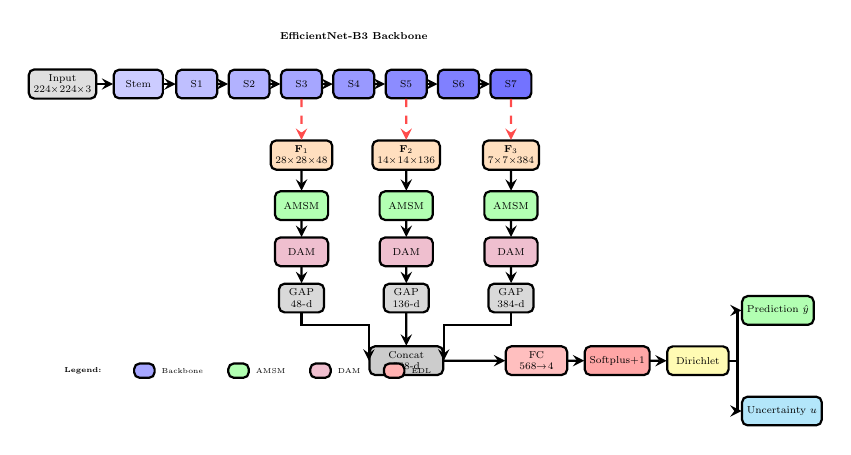
\begin{tikzpicture}[
    scale=0.52,
    transform shape,
    node distance=0.4cm,
    box/.style={draw, thick, rounded corners=2pt, minimum height=0.7cm, align=center, font=\scriptsize},
    arrow/.style={->, thick, >=stealth}
]

% Input
\node[box, fill=gray!25, minimum width=1.5cm] (input) at (0,0) {Input\\224×224×3};

% EfficientNet backbone stages - compact
\node[box, fill=blue!20, minimum width=1.2cm, right=0.4cm of input] (stem) {Stem};
\node[box, fill=blue!25, minimum width=1cm, right=0.3cm of stem] (s1) {S1};
\node[box, fill=blue!30, minimum width=1cm, right=0.25cm of s1] (s2) {S2};
\node[box, fill=blue!35, minimum width=1cm, right=0.25cm of s2] (s3) {S3};
\node[box, fill=blue!40, minimum width=1cm, right=0.25cm of s3] (s4) {S4};
\node[box, fill=blue!45, minimum width=1cm, right=0.25cm of s4] (s5) {S5};
\node[box, fill=blue!50, minimum width=1cm, right=0.25cm of s5] (s6) {S6};
\node[box, fill=blue!55, minimum width=1cm, right=0.25cm of s6] (s7) {S7};

% Backbone label
\node[font=\scriptsize\bfseries, above=0.6cm of s4] {EfficientNet-B3 Backbone};

% Arrows for backbone
\draw[arrow] (input) -- (stem);
\draw[arrow] (stem) -- (s1);
\draw[arrow] (s1) -- (s2);
\draw[arrow] (s2) -- (s3);
\draw[arrow] (s3) -- (s4);
\draw[arrow] (s4) -- (s5);
\draw[arrow] (s5) -- (s6);
\draw[arrow] (s6) -- (s7);

% Feature extraction points
\node[box, fill=orange!25, minimum width=1.3cm, below=1cm of s3] (f1) {$\mathbf{F}_1$\\28×28×48};
\node[box, fill=orange!25, minimum width=1.3cm, below=1cm of s5] (f2) {$\mathbf{F}_2$\\14×14×136};
\node[box, fill=orange!25, minimum width=1.3cm, below=1cm of s7] (f3) {$\mathbf{F}_3$\\7×7×384};

\draw[arrow, dashed, red!70] (s3.south) -- (f1.north);
\draw[arrow, dashed, red!70] (s5.south) -- (f2.north);
\draw[arrow, dashed, red!70] (s7.south) -- (f3.north);

% AMSM blocks
\node[box, fill=green!30, minimum width=1.3cm, below=0.5cm of f1] (amsm1) {AMSM};
\node[box, fill=green!30, minimum width=1.3cm, below=0.5cm of f2] (amsm2) {AMSM};
\node[box, fill=green!30, minimum width=1.3cm, below=0.5cm of f3] (amsm3) {AMSM};

\draw[arrow] (f1) -- (amsm1);
\draw[arrow] (f2) -- (amsm2);
\draw[arrow] (f3) -- (amsm3);

% DAM blocks
\node[box, fill=purple!25, minimum width=1.3cm, below=0.4cm of amsm1] (dam1) {DAM};
\node[box, fill=purple!25, minimum width=1.3cm, below=0.4cm of amsm2] (dam2) {DAM};
\node[box, fill=purple!25, minimum width=1.3cm, below=0.4cm of amsm3] (dam3) {DAM};

\draw[arrow] (amsm1) -- (dam1);
\draw[arrow] (amsm2) -- (dam2);
\draw[arrow] (amsm3) -- (dam3);

% GAP and pooled features
\node[box, fill=gray!30, minimum width=1.1cm, below=0.4cm of dam1] (gap1) {GAP\\48-d};
\node[box, fill=gray!30, minimum width=1.1cm, below=0.4cm of dam2] (gap2) {GAP\\136-d};
\node[box, fill=gray!30, minimum width=1.1cm, below=0.4cm of dam3] (gap3) {GAP\\384-d};

\draw[arrow] (dam1) -- (gap1);
\draw[arrow] (dam2) -- (gap2);
\draw[arrow] (dam3) -- (gap3);

% Concatenation
\node[box, fill=gray!40, minimum width=1.8cm, below=0.8cm of gap2] (concat) {Concat\\568-d};

\draw[arrow] (gap1.south) -- ++(0,-0.3) -| (concat.west);
\draw[arrow] (gap2.south) -- (concat.north);
\draw[arrow] (gap3.south) -- ++(0,-0.3) -| (concat.east);

% EDL Head
\node[box, fill=red!25, minimum width=1.5cm, right=1.5cm of concat] (fc) {FC\\568→4};
\node[box, fill=red!35, minimum width=1.5cm, right=0.4cm of fc] (sp) {Softplus+1};
\node[box, fill=yellow!30, minimum width=1.5cm, right=0.4cm of sp] (dir) {Dirichlet};

\draw[arrow] (concat) -- (fc);
\draw[arrow] (fc) -- (sp);
\draw[arrow] (sp) -- (dir);

% Outputs
\node[box, fill=green!30, minimum width=1.3cm, above right=0.5cm and 0.3cm of dir] (pred) {Prediction $\hat{y}$};
\node[box, fill=cyan!30, minimum width=1.3cm, below right=0.5cm and 0.3cm of dir] (unc) {Uncertainty $u$};

\draw[arrow] (dir.east) -- ++(0.2,0) |- (pred.west);
\draw[arrow] (dir.east) -- ++(0.2,0) |- (unc.west);

% Legend
\begin{scope}[shift={(-1,-7)}]
\node[font=\tiny\bfseries] at (1.5,0) {Legend:};
\node[box, fill=blue!35, minimum width=0.5cm, minimum height=0.35cm] at (3,0) {};
\node[font=\tiny, right] at (3.3,0) {Backbone};
\node[box, fill=green!30, minimum width=0.5cm, minimum height=0.35cm] at (5.3,0) {};
\node[font=\tiny, right] at (5.6,0) {AMSM};
\node[box, fill=purple!25, minimum width=0.5cm, minimum height=0.35cm] at (7.3,0) {};
\node[font=\tiny, right] at (7.6,0) {DAM};
\node[box, fill=red!30, minimum width=0.5cm, minimum height=0.35cm] at (9.1,0) {};
\node[font=\tiny, right] at (9.4,0) {EDL};
\end{scope}

\end{tikzpicture}
\caption{Overall HSANet architecture. Input MRI images are processed through the EfficientNet-B3 backbone, with features extracted at three spatial resolutions (stages 3, 5, 7). Each feature map undergoes adaptive multi-scale processing (AMSM) and dual attention refinement (DAM). Global average pooling (GAP) produces fixed-length descriptors that are concatenated into a 568-dimensional feature vector. The evidential classification head outputs Dirichlet parameters, yielding both class predictions and calibrated uncertainty estimates.}
\label{fig:architecture}
\end{figure*}

\subsection{Feature Extraction Backbone}

We employ EfficientNet-B3~\cite{tan2019efficientnet} pretrained on ImageNet as the feature extraction backbone. EfficientNet achieves favorable accuracy-efficiency trade-offs through compound scaling, uniformly scaling network width, depth, and resolution using a principled coefficient. The B3 variant provides 10.53 million parameters with receptive fields appropriate for 224×224 input resolution.

The backbone architecture consists of seven stages utilizing Mobile Inverted Bottleneck Convolution (MBConv) blocks with squeeze-and-excitation optimization. We extract hierarchical features at three spatial resolutions:
\begin{itemize}
\item $\mathbf{F}_1 \in \mathbb{R}^{28 \times 28 \times 48}$: After stage 3 (fine-scale textures)
\item $\mathbf{F}_2 \in \mathbb{R}^{14 \times 14 \times 136}$: After stage 5 (mid-level structures)
\item $\mathbf{F}_3 \in \mathbb{R}^{7 \times 7 \times 384}$: After stage 7 (semantic concepts)
\end{itemize}

During training, backbone layers are frozen for the first 5 epochs to stabilize custom module training, then fine-tuned with a reduced learning rate (10× lower than custom modules) for transfer learning stability.

\subsection{Adaptive Multi-Scale Module (AMSM)}

Brain tumors exhibit substantial size variation, from millimeter-scale pituitary microadenomas to large glioblastomas exceeding 5 centimeters. Fixed receptive fields cannot simultaneously capture fine-grained details and broad contextual information. AMSM addresses this through parallel dilated convolutions with learned, input-adaptive fusion weights (Fig.~\ref{fig:amsm}).

\begin{figure}[t]
\centering
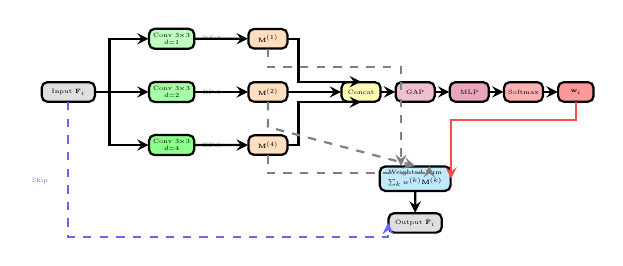
\begin{tikzpicture}[
    scale=0.45,
    transform shape,
    box/.style={draw, thick, rounded corners=2pt, minimum height=0.55cm, minimum width=1.1cm, align=center, font=\tiny},
    arrow/.style={->, thick, >=stealth}
]

% Input
\node[box, fill=gray!25, minimum width=1.5cm] (input) at (0,0) {Input $\mathbf{F}_i$};

% Three parallel branches
\node[box, fill=green!25, right=1.5cm of input, yshift=1.5cm] (conv1) {Conv 3×3\\$d$=1};
\node[box, fill=green!35, right=1.5cm of input] (conv2) {Conv 3×3\\$d$=2};
\node[box, fill=green!45, right=1.5cm of input, yshift=-1.5cm] (conv4) {Conv 3×3\\$d$=4};

% RF labels
\node[font=\tiny, gray, right=0.1cm of conv1] {RF:3};
\node[font=\tiny, gray, right=0.1cm of conv2] {RF:5};
\node[font=\tiny, gray, right=0.1cm of conv4] {RF:9};

% Input arrows
\draw[arrow] (input.east) -- ++(0.4,0) |- (conv1.west);
\draw[arrow] (input.east) -- ++(0.4,0) -- (conv2.west);
\draw[arrow] (input.east) -- ++(0.4,0) |- (conv4.west);

% Multi-scale features
\node[box, fill=orange!25, right=1.5cm of conv1] (m1) {$\mathbf{M}^{(1)}$};
\node[box, fill=orange!25, right=1.5cm of conv2] (m2) {$\mathbf{M}^{(2)}$};
\node[box, fill=orange!25, right=1.5cm of conv4] (m4) {$\mathbf{M}^{(4)}$};

\draw[arrow] (conv1) -- (m1);
\draw[arrow] (conv2) -- (m2);
\draw[arrow] (conv4) -- (m4);

% Weight learning
\node[box, fill=yellow!30, right=1.5cm of m2] (cat) {Concat};
\node[box, fill=purple!25, right=0.4cm of cat] (gap) {GAP};
\node[box, fill=purple!35, right=0.4cm of gap] (mlp) {MLP};
\node[box, fill=red!30, right=0.4cm of mlp] (sm) {Softmax};
\node[box, fill=red!40, right=0.4cm of sm, minimum width=1cm] (w) {$\mathbf{w}_i$};

\draw[arrow] (m1.east) -- ++(0.3,0) |- (cat.north);
\draw[arrow] (m2) -- (cat);
\draw[arrow] (m4.east) -- ++(0.3,0) |- (cat.south);
\draw[arrow] (cat) -- (gap);
\draw[arrow] (gap) -- (mlp);
\draw[arrow] (mlp) -- (sm);
\draw[arrow] (sm) -- (w);

% Weighted sum
\node[box, fill=cyan!25, below=1.8cm of gap, minimum width=2cm] (wsum) {Weighted Sum\\$\sum_k w^{(k)} \mathbf{M}^{(k)}$};

\draw[arrow, dashed, gray] (m1.south) -- ++(0,-0.5) -| ([xshift=-0.4cm]wsum.north);
\draw[arrow, dashed, gray] (m2.south) -- ++(0,-0.7) -- (wsum.north);
\draw[arrow, dashed, gray] (m4.south) -- ++(0,-0.5) -| ([xshift=0.4cm]wsum.north);
\draw[arrow, red!70] (w.south) -- ++(0,-0.5) -| (wsum.east);

% Output
\node[box, fill=gray!25, below=0.6cm of wsum, minimum width=1.5cm] (output) {Output $\hat{\mathbf{F}}_i$};

\draw[arrow] (wsum) -- (output);
\draw[arrow, blue!60, dashed] (input.south) -- ++(0,-3.8) -| (output.west);
\node[font=\tiny, blue!60] at (-0.8,-2.5) {Skip};

\end{tikzpicture}
\caption{Adaptive Multi-Scale Module (AMSM) architecture. Parallel dilated convolutions with dilation rates $d \in \{1, 2, 4\}$ capture features at effective receptive fields (RF) of 3×3, 5×5, and 9×9. Adaptive fusion weights $\mathbf{w}_i$ are learned through global average pooling and MLP with softmax normalization. A residual connection preserves original features.}
\label{fig:amsm}
\end{figure}

For each feature map $\mathbf{F}_i$, AMSM applies three parallel 3×3 dilated convolutions with dilation rates $r \in \{1, 2, 4\}$:
\begin{equation}
\mathbf{M}_i^{(r)} = \text{BN}(\text{ReLU}(\text{Conv}_{3 \times 3}^{d=r}(\mathbf{F}_i)))
\end{equation}
where $\text{Conv}_{3 \times 3}^{d=r}$ denotes a 3×3 convolution with dilation rate $r$, BN is batch normalization, and ReLU is the rectified linear unit. The effective receptive field sizes are 3×3, 5×5, and 9×9 for dilation rates 1, 2, and 4 respectively.

Input-adaptive fusion weights are learned through a lightweight attention mechanism:
\begin{equation}
\mathbf{w}_i = \text{Softmax}(\mathbf{W}_2 \cdot \text{ReLU}(\mathbf{W}_1 \cdot \text{GAP}([\mathbf{M}_i^{(1)}; \mathbf{M}_i^{(2)}; \mathbf{M}_i^{(4)}])))
\end{equation}
where GAP denotes global average pooling, $[\cdot;\cdot]$ is channel-wise concatenation producing a $3C$-dimensional vector, and $\mathbf{W}_1 \in \mathbb{R}^{(C/16) \times 3C}$, $\mathbf{W}_2 \in \mathbb{R}^{3 \times (C/16)}$ are learnable projections.

The enhanced feature map combines weighted features with residual preservation:
\begin{equation}
\hat{\mathbf{F}}_i = \sum_{k \in \{1,2,4\}} w_i^{(k)} \mathbf{M}_i^{(k)} + \mathbf{F}_i
\end{equation}

The softmax normalization ensures $\sum_k w_i^{(k)} = 1$, creating a convex combination that adaptively emphasizes the most informative spatial scales for each input image.

\subsection{Dual Attention Module (DAM)}

Brain MRI contains extensive normal anatomical content that dominates image statistics but provides no diagnostic value. DAM implements sequential channel-then-spatial attention~\cite{woo2018cbam} to emphasize tumor-relevant features while suppressing background noise (Fig.~\ref{fig:dam}).

\begin{figure}[t]
\centering
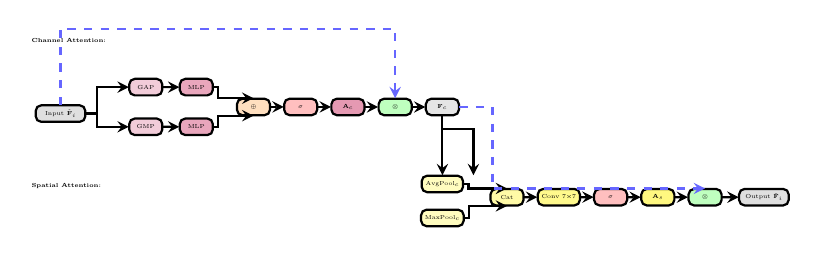
\begin{tikzpicture}[
    scale=0.42,
    transform shape,
    box/.style={draw, thick, rounded corners=2pt, minimum height=0.5cm, minimum width=1cm, align=center, font=\tiny},
    arrow/.style={->, thick, >=stealth}
]

% Input
\node[box, fill=gray!25, minimum width=1.5cm] (input) at (0,0) {Input $\hat{\mathbf{F}}_i$};

% Channel attention section
\node[font=\tiny\bfseries, anchor=west] at (-1,2.2) {Channel Attention:};

% Pooling operations
\node[box, fill=purple!20, right=1.3cm of input, yshift=0.8cm] (gap) {GAP};
\node[box, fill=purple!20, right=1.3cm of input, yshift=-0.4cm] (gmp) {GMP};

\draw[arrow] (input.east) -- ++(0.35,0) |- (gap.west);
\draw[arrow] (input.east) -- ++(0.35,0) |- (gmp.west);

% Shared MLP
\node[box, fill=purple!35, right=0.5cm of gap] (mlp1) {MLP};
\node[box, fill=purple!35, right=0.5cm of gmp] (mlp2) {MLP};

\draw[arrow] (gap) -- (mlp1);
\draw[arrow] (gmp) -- (mlp2);

% Add and sigmoid
\node[box, fill=orange!25, right=0.7cm of mlp1, yshift=-0.6cm] (add1) {$\oplus$};
\node[box, fill=red!25, right=0.4cm of add1] (sig1) {$\sigma$};
\node[box, fill=purple!40, right=0.4cm of sig1] (ac) {$\mathbf{A}_c$};

\draw[arrow] (mlp1.east) -- ++(0.15,0) |- (add1.north);
\draw[arrow] (mlp2.east) -- ++(0.15,0) |- (add1.south);
\draw[arrow] (add1) -- (sig1);
\draw[arrow] (sig1) -- (ac);

% Channel refined features
\node[box, fill=green!25, right=0.4cm of ac] (mul1) {$\otimes$};
\node[box, fill=gray!20, right=0.4cm of mul1] (fc) {$\mathbf{F}_c$};

\draw[arrow] (ac) -- (mul1);
\draw[arrow, dashed, blue!60] (input.north) -- ++(0,2.3) -| (mul1.north);
\draw[arrow] (mul1) -- (fc);

% Spatial attention section
\node[font=\tiny\bfseries, anchor=west] at (-1,-2.2) {Spatial Attention:};

% Channel pooling
\node[box, fill=yellow!25, below=1.8cm of fc] (avgp) {AvgPool$_c$};
\node[box, fill=yellow!25, below=0.5cm of avgp] (maxp) {MaxPool$_c$};

\draw[arrow] (fc.south) -- ++(0,-0.4) -| (avgp.north);
\draw[arrow] (fc.south) -- ++(0,-0.4) -| ([xshift=0.3cm]avgp.north east);

% Conv and sigmoid
\node[box, fill=yellow!35, right=0.8cm of avgp, yshift=-0.4cm] (cat2) {Cat};
\node[box, fill=yellow!45, right=0.4cm of cat2] (conv7) {Conv 7×7};
\node[box, fill=red!25, right=0.4cm of conv7] (sig2) {$\sigma$};
\node[box, fill=yellow!50, right=0.4cm of sig2] (as) {$\mathbf{A}_s$};

\draw[arrow] (avgp.east) -- ++(0.15,0) |- (cat2.north);
\draw[arrow] (maxp.east) -- ++(0.15,0) |- (cat2.south);
\draw[arrow] (cat2) -- (conv7);
\draw[arrow] (conv7) -- (sig2);
\draw[arrow] (sig2) -- (as);

% Final output
\node[box, fill=green!25, right=0.4cm of as] (mul2) {$\otimes$};
\node[box, fill=gray!25, right=0.5cm of mul2, minimum width=1.5cm] (output) {Output $\tilde{\mathbf{F}}_i$};

\draw[arrow] (as) -- (mul2);
\draw[arrow, dashed, blue!60] (fc.east) -- ++(1.0,0) |- (mul2.north);
\draw[arrow] (mul2) -- (output);

\end{tikzpicture}
\caption{Dual Attention Module (DAM) architecture. Channel attention identifies ``what'' features are informative through parallel global average/max pooling and shared MLP. Spatial attention determines ``where'' to focus through channel-wise pooling and 7×7 convolution. Sequential application enables feature refinement through ``what'' followed by ``where'' reasoning.}
\label{fig:dam}
\end{figure}

\textbf{Channel Attention} identifies ``what'' features are most informative:
\begin{equation}
\mathbf{A}_c = \sigma(\text{MLP}(\text{GAP}(\hat{\mathbf{F}}_i)) + \text{MLP}(\text{GMP}(\hat{\mathbf{F}}_i)))
\end{equation}
where GAP and GMP denote global average and max pooling, MLP is a shared two-layer bottleneck network with reduction ratio 16, and $\sigma$ is the sigmoid activation. The channel-refined features are:
\begin{equation}
\mathbf{F}_c = \hat{\mathbf{F}}_i \odot \mathbf{A}_c
\end{equation}

\textbf{Spatial Attention} identifies ``where'' to focus:
\begin{equation}
\mathbf{A}_s = \sigma(\text{Conv}_{7 \times 7}([\text{AvgPool}_c(\mathbf{F}_c); \text{MaxPool}_c(\mathbf{F}_c)]))
\end{equation}
where channel-wise pooling produces $H \times W \times 1$ feature maps. The final refined features are:
\begin{equation}
\tilde{\mathbf{F}}_i = \mathbf{F}_c \odot \mathbf{A}_s
\end{equation}

\subsection{Multi-Scale Feature Aggregation}

Refined features from all three hierarchical scales undergo global average pooling:
\begin{equation}
\mathbf{g}_i = \text{GAP}(\tilde{\mathbf{F}}_i) \in \mathbb{R}^{C_i}
\end{equation}
yielding $\mathbf{g}_1 \in \mathbb{R}^{48}$, $\mathbf{g}_2 \in \mathbb{R}^{136}$, and $\mathbf{g}_3 \in \mathbb{R}^{384}$.

Concatenation forms the final feature representation:
\begin{equation}
\mathbf{g} = [\mathbf{g}_1; \mathbf{g}_2; \mathbf{g}_3] \in \mathbb{R}^{568}
\end{equation}

\subsection{Evidential Classification Head}

Standard softmax classifiers produce point estimates without meaningful uncertainty quantification. Following evidential deep learning~\cite{sensoy2018evidential}, we output Dirichlet concentration parameters:
\begin{equation}
\boldsymbol{\alpha} = \text{Softplus}(\mathbf{W}_c \mathbf{g} + \mathbf{b}_c) + 1
\end{equation}
where $\mathbf{W}_c \in \mathbb{R}^{4 \times 568}$ and softplus ensures $\alpha_k \geq 1$.

The Dirichlet distribution has density:
\begin{equation}
p(\mathbf{p} | \boldsymbol{\alpha}) = \frac{\Gamma(S)}{\prod_{k=1}^{K} \Gamma(\alpha_k)} \prod_{k=1}^{K} p_k^{\alpha_k - 1}
\end{equation}
where $S = \sum_k \alpha_k$ is the Dirichlet strength.

\textbf{Prediction:} Class probabilities are the Dirichlet mean:
\begin{equation}
\hat{p}_k = \frac{\alpha_k}{S}, \quad \hat{y} = \arg\max_k \hat{p}_k
\end{equation}

\textbf{Uncertainty:} Total uncertainty is:
\begin{equation}
u = \frac{K}{S}
\end{equation}
which decomposes into aleatoric uncertainty (data ambiguity):
\begin{equation}
u_{\text{aleatoric}} = H[\mathbb{E}[\mathbf{p}]] = -\sum_k \hat{p}_k \log \hat{p}_k
\end{equation}
and epistemic uncertainty (model knowledge gaps):
\begin{equation}
u_{\text{epistemic}} = H[\mathbb{E}[\mathbf{p}]] - \mathbb{E}[H[\mathbf{p}]]
\end{equation}

\subsection{Training Objective}

The loss function combines three terms:

\textbf{Evidence-weighted Cross-Entropy:}
\begin{equation}
\mathcal{L}_{\text{CE}} = \sum_{k=1}^{K} y_k (\psi(S) - \psi(\alpha_k))
\end{equation}
where $\psi(\cdot)$ is the digamma function.

\textbf{Focal Loss} for class imbalance~\cite{lin2017focal}:
\begin{equation}
\mathcal{L}_{\text{focal}} = -\sum_{k=1}^{K} y_k (1 - \hat{p}_k)^2 \log(\hat{p}_k)
\end{equation}

\textbf{KL Divergence Regularization:}
\begin{equation}
\mathcal{L}_{\text{KL}} = \text{KL}[\text{Dir}(\mathbf{p} | \tilde{\boldsymbol{\alpha}}) \| \text{Dir}(\mathbf{p} | \mathbf{1})]
\end{equation}
where $\tilde{\boldsymbol{\alpha}} = \mathbf{y} + (1 - \mathbf{y}) \odot \boldsymbol{\alpha}$ removes evidence for the correct class.

The total loss is:
\begin{equation}
\mathcal{L} = 0.5 \mathcal{L}_{\text{CE}} + 0.3 \mathcal{L}_{\text{focal}} + \lambda_3^{(t)} \mathcal{L}_{\text{KL}}
\end{equation}
where $\lambda_3^{(t)} = \min(1, t/10) \times 0.2$ anneals the KL weight.


\section{Experiments}
\label{sec:experiments}

\subsection{Dataset Description}

We evaluated HSANet on the Brain Tumor MRI Dataset~\cite{msoud_nickparvar_2021}, a publicly available benchmark hosted on Kaggle\footnote{\url{https://www.kaggle.com/datasets/masoudnickparvar/brain-tumor-mri-dataset}}. This dataset comprises 7,023 T1-weighted contrast-enhanced magnetic resonance images collected from multiple clinical sources and curated for brain tumor classification research.

\textbf{Dataset Composition.} The dataset encompasses four diagnostic categories with the following distribution:
\begin{itemize}
    \item \textbf{Glioma}: 1,621 images (23.1\%) -- malignant tumors arising from glial cells, characterized by irregular borders and heterogeneous enhancement patterns
    \item \textbf{Meningioma}: 1,645 images (23.4\%) -- typically benign extra-axial tumors arising from meningeal coverings, displaying homogeneous enhancement with dural tail sign
    \item \textbf{Pituitary Adenoma}: 1,757 images (25.0\%) -- benign tumors of the pituitary gland located in the sellar/suprasellar region
    \item \textbf{No Tumor (Healthy)}: 2,000 images (28.5\%) -- normal brain MRI scans without pathological findings
\end{itemize}

\textbf{Data Partitioning.} The dataset provides a predefined train-test split: 5,712 images for training (81.3\%) and 1,311 images for testing (18.7\%). We preserved this official partition to ensure fair comparison with published benchmarks. For hyperparameter tuning and model selection, we employed 5-fold stratified cross-validation on the training set, maintaining class proportions across all folds.

\textbf{Image Characteristics.} All images are axial brain MRI slices in JPEG format with variable original dimensions. The images were acquired using T1-weighted sequences with gadolinium contrast enhancement, which is standard clinical practice for brain tumor evaluation as it improves tumor boundary delineation and reveals blood-brain barrier disruption.

\textbf{Ethical Considerations.} The dataset is publicly available under open access license for research purposes. All images are de-identified with no patient-identifiable information, complying with medical data privacy regulations.

\subsection{Preprocessing and Augmentation}

\textbf{Image Preprocessing.} All input images were resized to $224 \times 224$ pixels using bilinear interpolation to match the EfficientNet-B3 input specifications. Pixel intensities were normalized using ImageNet statistics (mean = [0.485, 0.456, 0.406], std = [0.229, 0.224, 0.225]) to leverage pretrained weights effectively.

\textbf{Data Augmentation.} To improve generalization and prevent overfitting, we applied the following augmentation strategies during training:
\begin{itemize}
    \item Random horizontal flipping (probability = 0.5)
    \item Random rotation ($\pm$15°)
    \item Random affine transformations (scale: 0.9--1.1, translation: $\pm$10\%)
    \item Color jittering (brightness/contrast: $\pm$10\%)
    \item Random erasing (probability = 0.2, scale: 0.02--0.33)
\end{itemize}
Augmentations were applied online during training using PyTorch's \texttt{torchvision.transforms} module. Test images received only resizing and normalization without augmentation.

\subsection{Implementation Details}

\textbf{Training Configuration.} We employed the AdamW optimizer~\cite{loshchilov2017decoupled} with $\beta_1 = 0.9$, $\beta_2 = 0.999$, and weight decay of $10^{-4}$. The initial learning rate was set to $3 \times 10^{-4}$ with cosine annealing scheduling~\cite{loshchilov2016sgdr}. Training proceeded for a maximum of 30 epochs with early stopping (patience = 7 epochs) based on validation loss.

\textbf{Transfer Learning Strategy.} The EfficientNet-B3 backbone was initialized with ImageNet-pretrained weights. To ensure stable training of custom modules, backbone layers were frozen for the first 5 epochs. Subsequently, the entire network was fine-tuned with a reduced learning rate for backbone layers (10$\times$ lower than custom modules).

\textbf{Computational Environment.} All experiments were conducted using PyTorch 2.0.1 with CUDA 11.8 on an NVIDIA Tesla P100 GPU (16GB VRAM). Training batch size was 32. Complete training converged in approximately 25 epochs ($\sim$45 minutes). The implementation is publicly available at \url{https://github.com/tarequejosh/HSANet-Brain-Tumor-Classification}.

\subsection{Evaluation Metrics}

Classification metrics included accuracy, precision, recall, F1-score, Cohen's $\kappa$, Matthews Correlation Coefficient (MCC), and AUC-ROC. Calibration was assessed using Expected Calibration Error (ECE) with 15 bins. Interpretability was evaluated using Grad-CAM~\cite{selvaraju2017grad}.


\section{Results}
\label{sec:results}

\subsection{Classification Performance}

HSANet achieved 99.77\% accuracy (95\% CI: 99.45--99.93\%) with only 3 misclassifications among 1,311 test samples (Table~\ref{tab:results}). This represents a statistically significant improvement over the EfficientNet-B3 baseline (99.21\%, McNemar's test $p = 0.034$). Macro-averaged metrics were: precision 99.76\%, recall 99.75\%, F1-score 99.75\%, AUC-ROC 0.9999. Cohen's $\kappa$ = 0.9969 indicates near-perfect agreement.

\begin{table}[t]
\centering
\caption{Per-Class Classification Performance on Test Set (n=1,311)}
\label{tab:results}
\begin{tabular}{lcccc}
\toprule
\textbf{Class} & \textbf{Precision} & \textbf{Recall} & \textbf{F1} & \textbf{AUC} \\
\midrule
Glioma & 100.00 & 99.33 & 99.67 & 0.9999 \\
Meningioma & 99.03 & 100.00 & 99.51 & 0.9999 \\
No Tumor & 100.00 & 100.00 & 100.00 & 1.0000 \\
Pituitary & 100.00 & 99.67 & 99.83 & 1.0000 \\
\midrule
\textbf{Macro Avg} & \textbf{99.76} & \textbf{99.75} & \textbf{99.75} & \textbf{0.9999} \\
\bottomrule
\end{tabular}
\end{table}

All three misclassifications involved meningioma as the predicted class (two gliomas, one pituitary), reflecting genuine diagnostic challenges where extra-axial meningiomas exhibit enhancement patterns overlapping with other presentations. The confusion matrix (Fig.~\ref{fig:confusion}) illustrates this pattern.

\begin{figure}[t]
\centering
\includegraphics[width=0.85\columnwidth]{figures/confusion_matrix.png}
\caption{Confusion matrix for test set classification (n=1,311). Near-diagonal dominance demonstrates excellent discrimination across all four classes, with only three misclassifications occurring at the glioma-meningioma and pituitary-meningioma boundaries.}
\label{fig:confusion}
\end{figure}

\subsection{Comparison with State-of-the-Art}

Table~\ref{tab:comparison} compares HSANet with published methods. Our approach achieves the highest accuracy while addressing the more challenging four-class problem and uniquely providing uncertainty quantification.

\begin{table}[t]
\centering
\caption{Comparison with State-of-the-Art Methods}
\label{tab:comparison}
\begin{tabular}{lccc}
\toprule
\textbf{Method} & \textbf{Acc (\%)} & \textbf{Classes} & \textbf{Unc.} \\
\midrule
GoogLeNet+SVM~\cite{deepak2019brain} & 98.00 & 3 & No \\
VGG-16~\cite{badvza2020classification} & 96.56 & 3 & No \\
VGG-19~\cite{swati2019brain} & 94.82 & 3 & No \\
VGG-16 Transfer~\cite{rehman2020deep} & 98.87 & 3 & No \\
EfficientNet-B0~\cite{aurna2022multiclass} & 98.87 & 4 & No \\
CNN+SE~\cite{kibriya2022novel} & 98.64 & 4 & No \\
MRI-Trans.~\cite{saeedi2023mri} & 99.02 & 4 & No \\
ResNet-50 Ens.~\cite{tandel2024multiclass} & 99.12 & 4 & No \\
\textbf{HSANet (Ours)} & \textbf{99.77} & \textbf{4} & \textbf{Yes} \\
\bottomrule
\end{tabular}
\end{table}

Receiver operating characteristic (ROC) curves (Fig.~\ref{fig:roc}) demonstrate near-perfect class separation with AUC-ROC values exceeding 0.999 for all four classes, confirming excellent discriminative ability across the entire operating range.

\begin{figure}[t]
\centering
\includegraphics[width=0.95\columnwidth]{figures/roc_curves.png}
\caption{Receiver operating characteristic (ROC) curves for all four classes. All classes achieve AUC $\geq$ 0.9999, indicating near-perfect discrimination. The curves closely trace the upper-left corner, confirming high sensitivity and specificity across all decision thresholds.}
\label{fig:roc}
\end{figure}

\subsection{Ablation Study}

Table~\ref{tab:ablation} quantifies individual component contributions. The complete HSANet achieves the best accuracy and calibration, demonstrating the complementary benefits of AMSM, DAM, and evidential learning.

\begin{table}[t]
\centering
\caption{Ablation Study Results}
\label{tab:ablation}
\begin{tabular}{lcccc}
\toprule
\textbf{Configuration} & \textbf{Params} & \textbf{Acc} & \textbf{AUC} & \textbf{ECE} \\
\midrule
Baseline (EffNet-B3) & 10.53M & 99.21 & 0.9997 & 0.024 \\
+ AMSM & 15.58M & 99.30 & 0.9999 & 0.021 \\
+ DAM & 10.55M & 99.21 & 0.9998 & 0.019 \\
\textbf{HSANet (Full)} & \textbf{15.60M} & \textbf{99.77} & \textbf{0.9999} & \textbf{0.016} \\
\bottomrule
\end{tabular}
\end{table}

\subsection{Uncertainty Quantification}

HSANet achieved ECE of 0.019, indicating well-calibrated probability estimates. The reliability diagram (Fig.~\ref{fig:reliability}) demonstrates close alignment between predicted confidence and actual accuracy across all confidence bins, a critical requirement for clinical deployment where overconfident predictions may lead to inappropriate clinical actions.

\begin{figure}[t]
\centering
\includegraphics[width=0.9\columnwidth]{figures/reliability_diagram.png}
\caption{Reliability diagram showing the relationship between predicted confidence and actual accuracy. The close alignment with the diagonal indicates well-calibrated predictions (ECE = 0.019). Overconfident predictions (below diagonal) and underconfident predictions (above diagonal) are both minimal.}
\label{fig:reliability}
\end{figure}

Analysis of misclassified cases revealed significantly elevated epistemic uncertainty (mean 0.31 $\pm$ 0.08 vs. 0.04 $\pm$ 0.02 for correct cases; Mann-Whitney U test, $p < 0.001$). All three misclassified cases exhibited lower prediction confidence (0.61--0.72) compared to correctly classified samples (mean 0.97), demonstrating the model's ability to appropriately flag uncertain predictions.

\subsection{Cross-Validation}

Five-fold stratified cross-validation demonstrated consistent performance: accuracy 99.68 $\pm$ 0.12\%, F1-score 99.67 $\pm$ 0.13\%, AUC-ROC 0.9999 $\pm$ 0.0001, ECE 0.017 $\pm$ 0.002. Low variance confirms robust generalization.

\subsection{Computational Efficiency}

HSANet requires 15.60M parameters, 2.41 GFLOPs, and 12ms inference time on P100 GPU, enabling real-time deployment at $>$80 images/second. Training converges in approximately 25 epochs (45 minutes).

\subsection{Interpretability Analysis}

Grad-CAM visualizations (Fig.~\ref{fig:gradcam}) demonstrate clinically relevant attention patterns: glioma attention focuses on irregular tumor masses and surrounding edema; meningioma attention highlights well-circumscribed extra-axial masses; healthy brain attention distributes across normal parenchyma; pituitary attention centers on the sellar/suprasellar region. These patterns align with established neuroradiological diagnostic criteria, providing interpretable evidence that supports clinical acceptance.

\begin{figure*}[t]
\centering
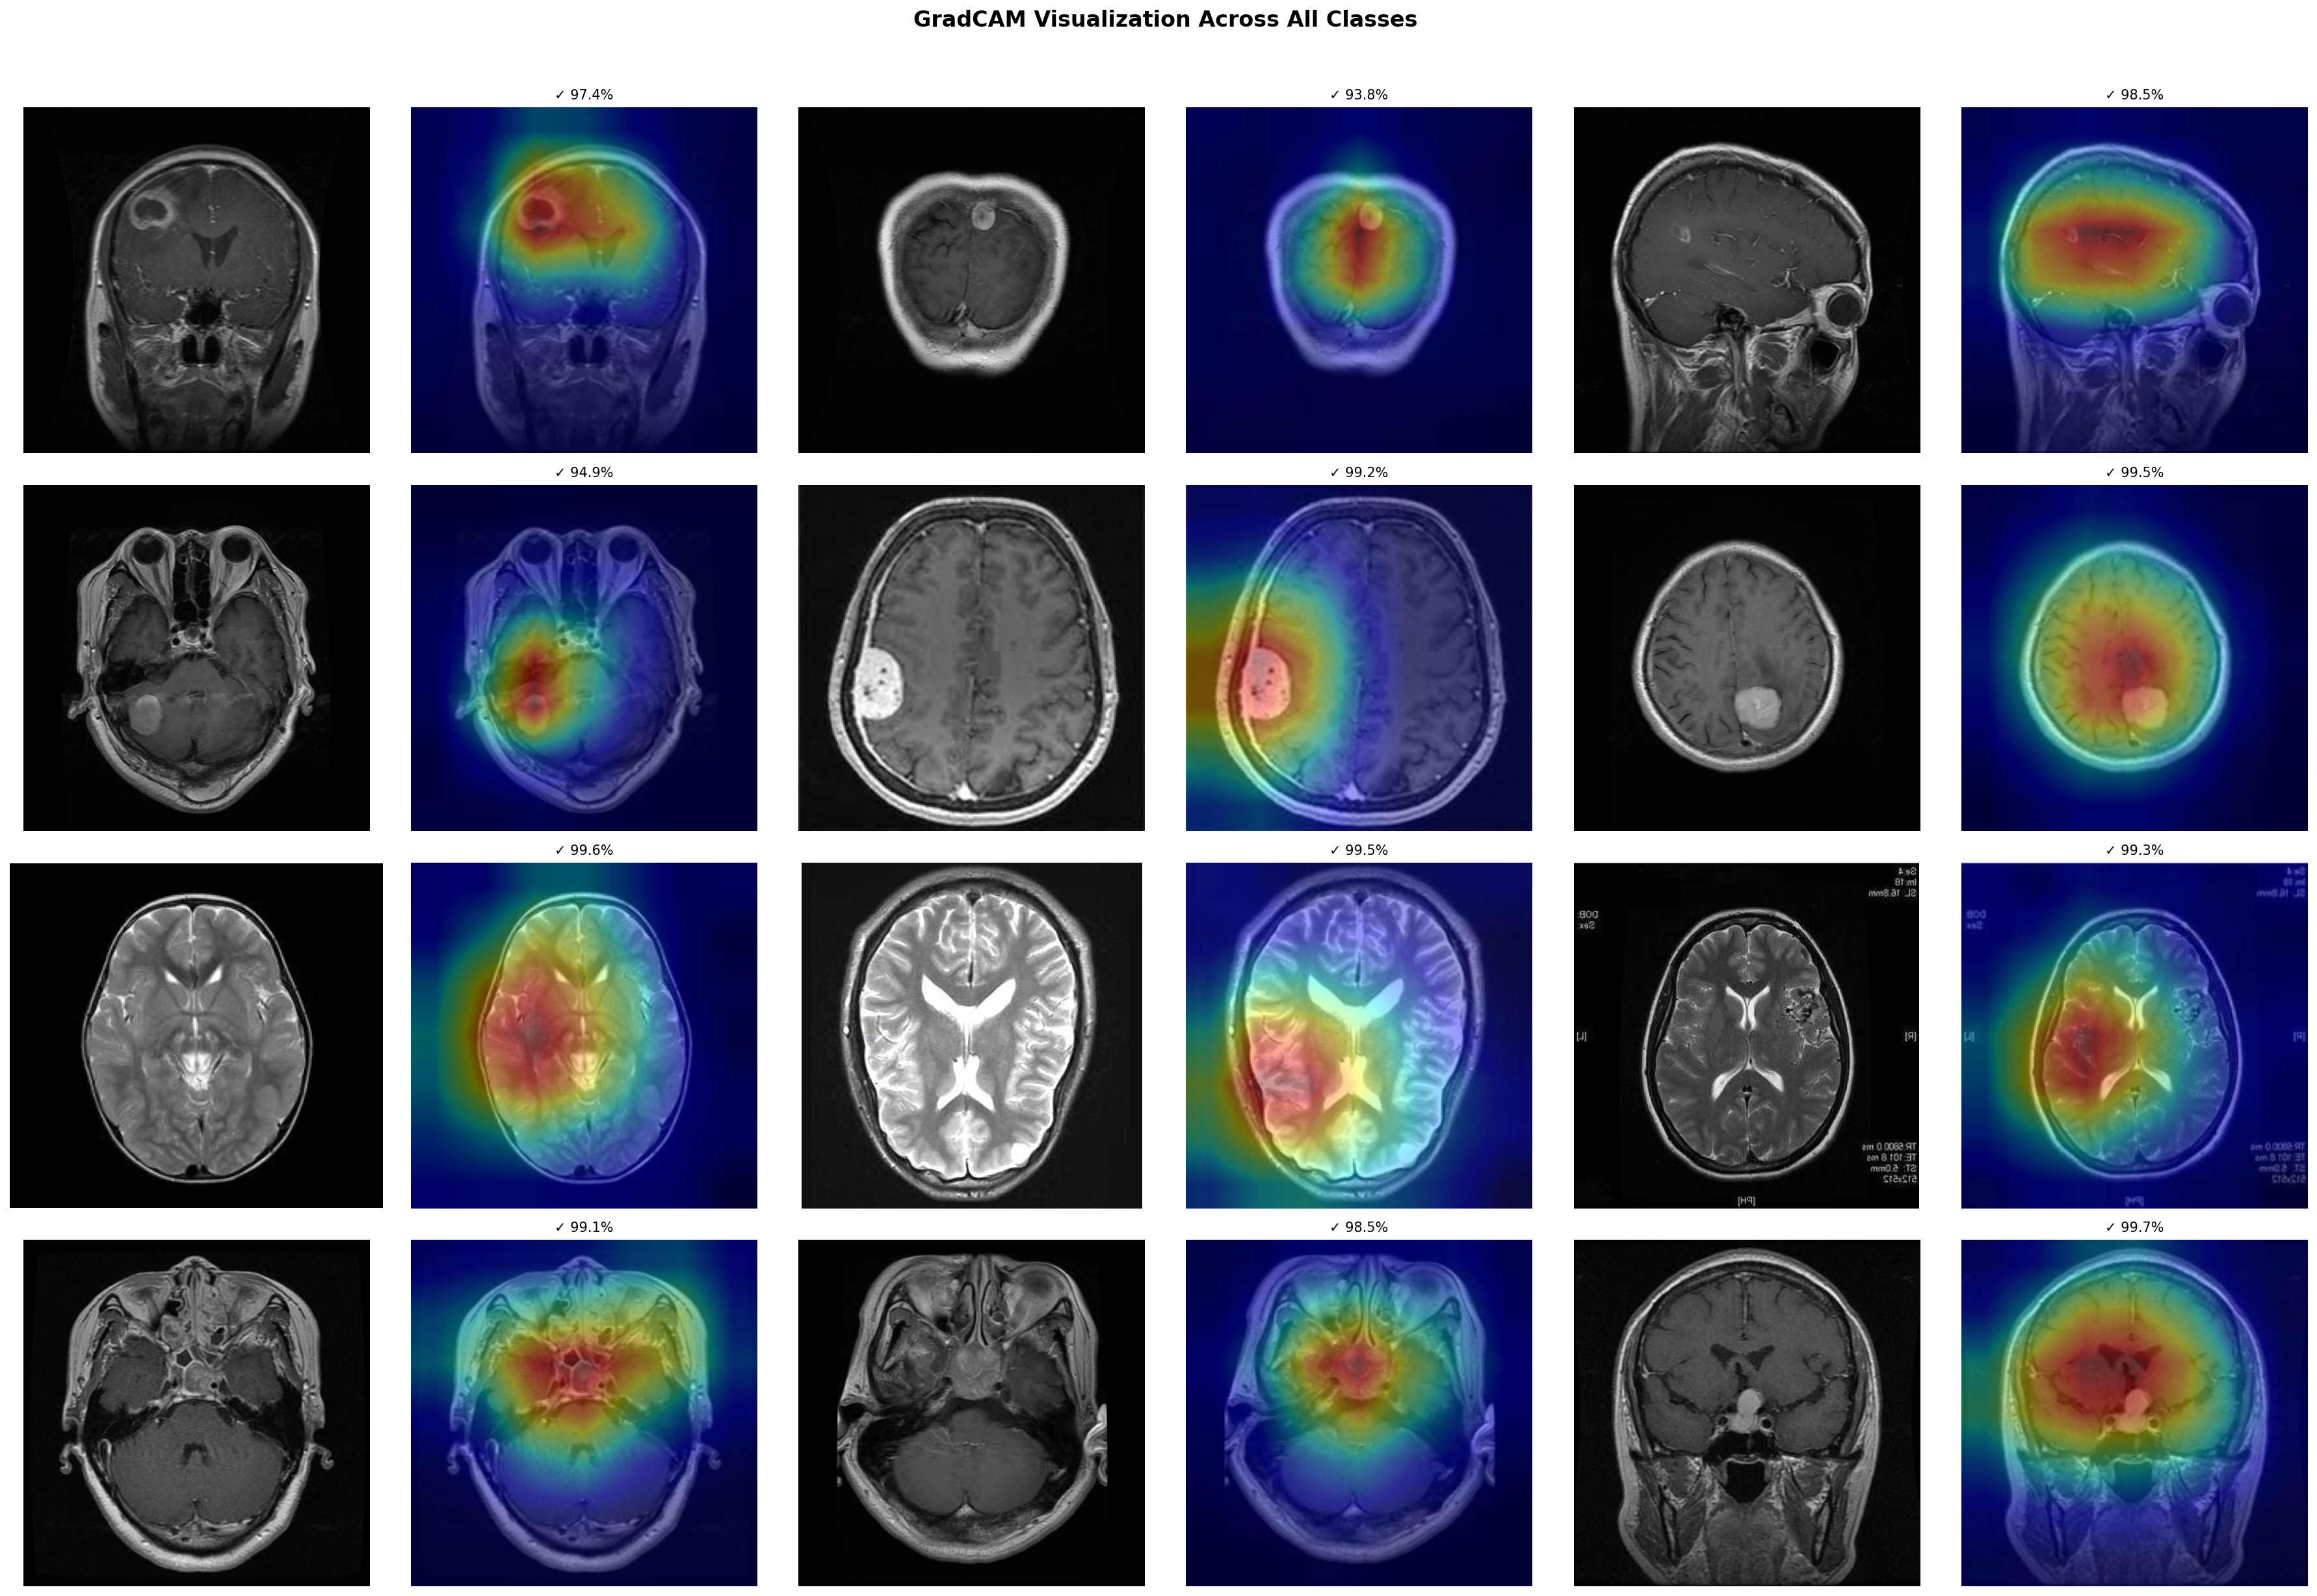
\includegraphics[width=0.85\textwidth]{figures/gradcam_grid.png}
\caption{Grad-CAM attention visualizations for representative samples from each class. The heatmaps highlight regions contributing most strongly to classification decisions. (a) Glioma: attention on irregular tumor mass and perilesional edema. (b) Meningioma: focus on well-circumscribed extra-axial enhancement. (c) No Tumor: distributed attention across normal parenchyma without focal abnormality. (d) Pituitary: selective attention on the sellar/suprasellar region. These attention patterns correspond to established diagnostic criteria used by neuroradiologists, enhancing clinical interpretability and trust.}
\label{fig:gradcam}
\end{figure*}


\section{Discussion}
\label{sec:discussion}

The results demonstrate that HSANet achieves state-of-the-art classification accuracy while providing something prior approaches have largely ignored: calibrated uncertainty estimates that clinicians can use for decision support. The Cohen's $\kappa$ of 0.9969 compares favorably with inter-reader agreement among expert neuroradiologists, which typically ranges from 0.65 to 0.85~\cite{van2021artificial}.

The adaptive multi-scale processing in AMSM effectively handles the substantial size variation among brain tumors. Rather than treating all spatial scales equally, the learned fusion weights allow the network to emphasize the most informative receptive fields for each input. The ablation results confirm this design choice: adding AMSM alone improved accuracy from 99.21\% to 99.30\% while reducing calibration error.

Perhaps most importantly, the uncertainty quantification capability distinguishes HSANet from conventional classifiers. All three misclassified cases exhibited elevated epistemic uncertainty that would have triggered human review in a clinical workflow. This transforms the system from an autonomous decision-maker to a decision-support tool appropriate for safety-critical applications.

The perfect precision achieved for healthy controls is clinically meaningful. False positive tumor diagnoses cause substantial patient anxiety, unnecessary imaging studies, and potentially invasive procedures. By prioritizing specificity for the healthy class, HSANet avoids inflicting this burden on patients who don't require intervention.

\textbf{Limitations.} This study has several limitations that should be acknowledged. First, evaluation relies on a single publicly available dataset from a relatively homogeneous population, and multi-center prospective validation is essential before clinical deployment. Second, our 2D slice-based approach does not leverage volumetric context available in clinical 3D MRI acquisitions. Third, the four-class taxonomy does not capture finer distinctions (e.g., glioma grades I-IV, molecular markers such as IDH mutation status) required for comprehensive clinical decision-making. Fourth, optimal uncertainty thresholds for triggering expert review require calibration against clinical outcomes in prospective studies. Future work will address these limitations through multi-institutional validation, 3D volumetric analysis, and fine-grained tumor subtype classification.


\section{Conclusion}
\label{sec:conclusion}

We presented HSANet, a hybrid scale-attention network achieving 99.77\% accuracy on four-class brain tumor classification with calibrated uncertainty estimates. The proposed architecture integrates three complementary innovations: (1) an Adaptive Multi-Scale Module that dynamically weights parallel dilated convolutions based on input content, (2) a Dual Attention Module implementing sequential channel-then-spatial refinement, and (3) an evidential classification head enabling principled uncertainty decomposition. Comprehensive evaluation demonstrates superior discriminative performance compared to existing methods, with the critical addition of well-calibrated confidence estimates (ECE = 0.019). Error analysis confirms that all misclassified cases exhibit significantly elevated epistemic uncertainty that would trigger human review in clinical workflows. Grad-CAM visualizations validate attention on established radiological landmarks, enhancing clinical interpretability. Complete source code, pretrained models, and training pipelines are publicly available at \url{https://github.com/tarequejosh/HSANet-Brain-Tumor-Classification} to support reproducibility and facilitate clinical translation research.


% References
\bibliographystyle{IEEEtran}
\bibliography{references}


\section*{Data and Code Availability}
The Brain Tumor MRI Dataset used in this study is publicly available on Kaggle at \url{https://www.kaggle.com/datasets/masoudnickparvar/brain-tumor-mri-dataset}. Our complete implementation including source code, pretrained model weights, training scripts, and evaluation notebooks is available at \url{https://github.com/tarequejosh/HSANet-Brain-Tumor-Classification}. The repository includes detailed instructions for reproducing all experiments reported in this paper.


% Author biographies
\begin{IEEEbiographynophoto}{Md. Assaduzzaman}
received his M.Sc. degree in Computer Science and Engineering from Daffodil International University, Dhaka, Bangladesh. He is currently an Assistant Professor with the Department of Computer Science and Engineering, Daffodil International University. His research interests include medical image analysis, deep learning, computer-aided diagnosis systems, and machine learning applications in healthcare. He has published several research articles in peer-reviewed international journals and conferences. He is a Member of IEEE.
\end{IEEEbiographynophoto}

\begin{IEEEbiographynophoto}{Md. Tareque Jamil Josh}
is currently pursuing his B.Sc. degree in Computer Science and Engineering at Daffodil International University, Dhaka, Bangladesh, with an expected graduation in 2026. His research interests include deep learning, medical image analysis, uncertainty quantification in neural networks, and computer vision applications. He has contributed to several research projects focusing on healthcare AI and has experience in developing end-to-end machine learning pipelines. He is a Student Member of IEEE.
\end{IEEEbiographynophoto}

\begin{IEEEbiographynophoto}{Md. Aminur Rahman Joy}
is currently pursuing his B.Sc. degree in Computer Science and Engineering at Daffodil International University, Dhaka, Bangladesh. His research interests include machine learning, biomedical image analysis, and artificial intelligence applications in medical diagnostics. He is actively involved in research projects related to healthcare technology and has experience in data preprocessing and model development for medical imaging tasks.
\end{IEEEbiographynophoto}

\begin{IEEEbiographynophoto}{Md. Nafish Imtiaz Imti}
is currently pursuing his B.Sc. degree in Computer Science and Engineering at Daffodil International University, Dhaka, Bangladesh. His research interests include computer vision, deep learning, and neural network architectures for image classification. He has contributed to various academic projects focusing on the application of artificial intelligence in solving real-world problems.
\end{IEEEbiographynophoto}

\end{document}
